\documentclass[11pt,a4paper]{article}

% --- Packages ---
\usepackage[margin=2.5cm]{geometry}
\usepackage[utf8]{inputenc}
\usepackage[T1]{fontenc}
\usepackage{lmodern}
\usepackage{graphicx}
\usepackage{booktabs}
\usepackage{tabularx}
\usepackage{multirow}
\usepackage{amsmath}
\usepackage{hyperref}
\usepackage{xcolor}
\usepackage{float}
\usepackage{caption}
\usepackage[numbers]{natbib}
\usepackage{enumitem}

\hypersetup{colorlinks=true, linkcolor=blue!60!black, citecolor=blue!60!black, urlcolor=blue!60!black}

% Figure path
\graphicspath{{../output/}}

% --- Title ---
\title{%
  \textbf{Skin Disease Classification}\\[0.5em]
  \large Applied Deep Learning --- Group Project Report\\[0.3em]
  \normalsize Group 3 --- Summer Semester 2026
}
\author{%
  Thilina Ranmal Angunna Gamage \and
  David Nunez Nepomuceno \and
  Diana Katonova \and
  Md Nahidul Islam\\[0.5em]
  \normalsize University of Graz
}
\date{\today}

\begin{document}
\maketitle
\tableofcontents
\newpage

% ======================================================================
% SECTION 1 — THILINA
% ======================================================================
\section{Project Setting and Goals}
\label{sec:setting}

% ---------------------------------------------------------------
% THILINA: Write this section (~1.5 pages). Guidelines below.
% ---------------------------------------------------------------

\subsection{Problem Context}
% THILINA: Cover these points:
% - Dermatological diagnosis is subjective and relies on expert pattern recognition
% - Access to dermatologists is limited globally (WHO statistics if available)
% - Automated skin disease classification from images is an active research area
% - Clinical decision-support tools could improve triage, especially in primary care
% - Key challenge: high inter-class visual similarity (e.g. eczema vs psoriasis)
% - Key challenge: intra-class variability (same disease looks very different across
%   skin tones, body locations, severity stages)
%
% Keep it concise. 1 paragraph of clinical motivation, 1 paragraph on the ML framing.

\textit{[To be written by Thilina]}

\subsection{Project Objectives}
% THILINA: Bullet list or short prose. Objectives are:
% 1. Build a multi-class image classifier for 18 dermatological conditions
% 2. Compare traditional ML baselines (RF, LogReg, SVM, KNN on pixel features)
%    against deep transfer learning (ResNet18, EfficientNet-B0)
% 3. Evaluate using balanced accuracy and macro F1 to account for class imbalance
% 4. Identify which disease classes remain difficult and discuss clinical implications
% 5. Produce a reproducible pipeline (numbered scripts, SLURM batch jobs, version-controlled)

\textit{[To be written by Thilina]}

\subsection{Related Work}
% THILINA: Cover 5-8 references. Suggested topics:
% - Transfer learning for skin lesion classification (Esteva et al. 2017, Nature)
% - ISIC challenge / HAM10000 dataset work (Tschandl et al. 2018)
% - EfficientNet and its use in medical imaging
% - Class imbalance handling in medical image classification
% - ResNet architecture (He et al. 2016) and why it transfers well
% - Any Kaggle skin disease dataset papers if available
%
% Format: 2-3 paragraphs grouping related work thematically.
% End with a sentence positioning our work relative to the literature.

\textit{[To be written by Thilina]}

% ======================================================================
% SECTION 2 — DAVID NUNEZ NEPOMUCENO (FULL PROSE)
% ======================================================================
\section{Dataset Description and Exploratory Analysis}
\label{sec:eda}

\subsection{Dataset Overview}

The dataset is a publicly available collection of dermatological images sourced from Kaggle, originally comprising 22 classes of skin conditions with a total of 15,444 images split into predefined training (13,898) and test (1,546) sets. Each class corresponds to a clinically recognised skin condition, ranging from common disorders such as acne and eczema to less prevalent conditions such as candidiasis and vasculitis. All images are provided as RGB photographs with heterogeneous resolutions, as the dataset aggregates clinical and dermoscopic images from multiple sources.

The predefined train/test split follows an approximate 90/10 ratio across all classes, indicating a stratified partitioning strategy. No official validation split is provided, and no patient-level identifiers are available, which limits the ability to enforce patient-level separation between splits. The dataset does not include metadata such as patient demographics, anatomical location or imaging device, which restricts the scope of bias analysis.

\subsection{Class Reduction: From 22 to 18 Classes}
\label{sec:class-reduction}

An initial transfer learning experiment using all 22 classes with ResNet18 and the identical training protocol described in Section~\ref{sec:transfer} yielded a balanced accuracy of 0.652 and a macro F1 of 0.637. Analysis of per-class recall revealed systematic weaknesses that motivated a principled reduction to 18 classes. Four classes were removed based on complementary clinical and statistical criteria:

Unknown/Normal, with 1,651 training images and a recall of 0.921, functions as a catch-all category for images that do not depict a specific skin disease. While the model classifies it with high recall, its inclusion introduces label noise. Visual inspection confirmed that this category contains non-dermatological images such as household objects and animals, indicating systematic label noise beyond clinical ambiguity. Furthermore, ``normal'' skin appearance varies widely across skin tones, ages and body regions, and the category boundary is defined by exclusion rather than by shared visual features. Removing it eliminates a source of distributional bias that disproportionately inflates overall accuracy without contributing to the diagnostic task.

Sun/Sunlight Damage, with 312 training images and a recall of 0.588, represents the early stage of a clinical continuum that includes actinic keratosis, a class retained in the dataset. The visual overlap between chronic sun damage and early actinic keratoses is substantial, as both present as rough, scaly patches on sun-exposed skin. Retaining both classes forces the model to learn a distinction that even dermatologists resolve through biopsy rather than visual inspection alone. With only 312 training images, the class lacks sufficient coverage to learn this subtle boundary.

Moles, with 361 training images and a recall of 0.525, present a classification challenge because the distinction between benign melanocytic naevi and early melanoma is the subject of dedicated binary classification systems in the literature. In a multi-class setting with 22 heterogeneous conditions, the model cannot learn the fine-grained features required for this distinction. At 0.525 recall, nearly half of mole images are misclassified, predominantly into the Skin Cancer and Benign Tumors categories. Including this class risks creating a false sense of diagnostic capability for a task that requires specialised architecture and data.

Lupus, with 311 training images and a recall of 0.471, encompasses multiple clinical subtypes: discoid lupus erythematosus, subacute cutaneous lupus and the malar rash of systemic lupus. These subtypes present with markedly different morphology. With only 311 images, the dataset cannot adequately represent this heterogeneity, resulting in the lowest recall among all classes. The visual overlap with rosacea, as both present with facial erythema, further compounds the classification difficulty.

\medskip

After removal, the reduced dataset comprises 18 classes with 11,263 training images and 1,249 test images. The class reduction improved balanced accuracy from 0.652 to 0.699, a gain of 4.7 percentage points, and macro F1 from 0.637 to 0.695, a gain of 5.8 points, under identical training conditions. This confirms that the removed classes were net contributors to classification noise rather than to diagnostic signal.

\subsection{Class Distribution and Imbalance}

Table~\ref{tab:class-dist} presents the distribution of images across the 18 retained classes. The largest class, Benign Tumors with 1,093 training images, contains approximately 4.4 times as many samples as the smallest, Candidiasis with 248 images. This moderate imbalance ratio is characteristic of medical imaging datasets, where disease prevalence varies across conditions.

\begin{table}[H]
\centering
\caption{Class distribution in the 18-class dataset, sorted by training set size.}
\label{tab:class-dist}
\small
\begin{tabular}{lrrr}
\toprule
\textbf{Class} & \textbf{Train} & \textbf{Test} & \textbf{Train \%} \\
\midrule
Benign Tumors       & 1,093 & 121 & 9.7 \\
Eczema              & 1,010 & 112 & 9.0 \\
Tinea               &   923 & 102 & 8.2 \\
Psoriasis           &   820 &  88 & 7.3 \\
Actinic Keratosis   &   748 &  83 & 6.6 \\
Vitiligo            &   714 &  82 & 6.3 \\
Skin Cancer         &   693 &  77 & 6.2 \\
Acne                &   593 &  65 & 5.3 \\
Warts               &   580 &  64 & 5.1 \\
Lichen              &   553 &  61 & 4.9 \\
Drug Eruption       &   547 &  61 & 4.9 \\
Vascular Tumors     &   543 &  60 & 4.8 \\
Infestations/Bites  &   524 &  60 & 4.7 \\
Bullous             &   504 &  55 & 4.5 \\
Vasculitis          &   461 &  52 & 4.1 \\
Seborrheic Keratoses&   455 &  51 & 4.0 \\
Rosacea             &   254 &  28 & 2.3 \\
Candidiasis         &   248 &  27 & 2.2 \\
\midrule
\textbf{Total}      & \textbf{11,263} & \textbf{1,249} & \textbf{100.0} \\
\bottomrule
\end{tabular}
\end{table}

To address class imbalance during training, we applied inverse-frequency weighting to the cross-entropy loss function: each class receives a weight proportional to the reciprocal of its sample count, normalised so that the weights sum to the number of classes. This approach penalises misclassification of minority classes more heavily without altering the training data distribution.

Figure~\ref{fig:class-dist} visualises this distribution.

\begin{figure}[H]
\centering
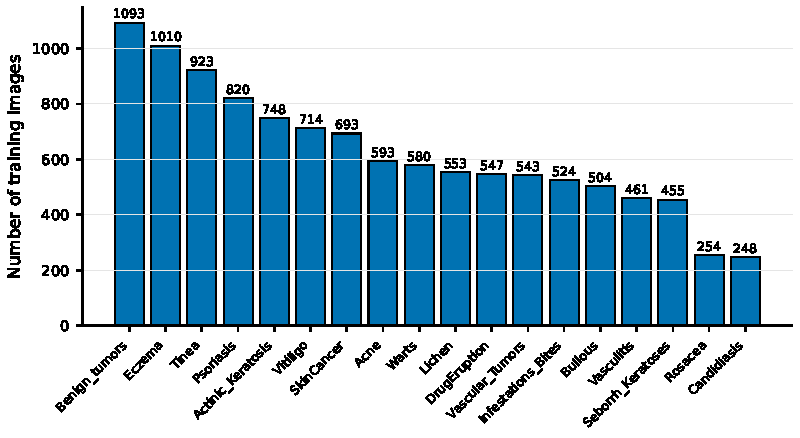
\includegraphics[width=0.95\textwidth]{eda/class_distribution.pdf}
\caption{Class distribution across the 18 retained classes, sorted by training set size.}
\label{fig:class-dist}
\end{figure}

\subsection{Image Properties}

All images are stored in RGB format with heterogeneous resolutions ranging from approximately 30 to over 4,000 pixels in both width and height, with a median of approximately 600 pixels. The majority of images have aspect ratios close to 1:1, which permits uniform resizing to 224$\times$224 pixels for transfer learning models and 32$\times$32 for traditional ML baselines with only moderate distortion. Per-class analysis of mean channel intensities shows that classes such as Vitiligo and Rosacea exhibit characteristic colour signatures, while classes such as Tinea and Eczema overlap substantially in colour space.

\subsection{Visual Inspection}

Figure~\ref{fig:samples} displays representative training images for each class. Several observations are relevant for classification:

\begin{itemize}[nosep]
  \item High intra-class variability: conditions such as Infestations/Bites and Drug Eruption encompass visually disparate presentations, ranging from insect bites to scabies and from maculopapular to urticarial reactions.
  \item Inter-class similarity: Eczema and Psoriasis both present as erythematous, scaly patches; Actinic Keratosis and Skin Cancer share morphological features on sun-damaged skin; Bullous diseases and Drug Eruptions can both manifest as blistering lesions.
  \item Imaging heterogeneity: the dataset mixes clinical photographs, including full-body and regional views, with close-up dermoscopic images, introducing scale and context variability within classes.
  \item Distinctive classes: Vitiligo with its characteristic depigmentation, Acne with comedones and pustules on facial skin, and Warts with verrucous texture exhibit strong visual signatures that facilitate classification.
\end{itemize}

\begin{figure}[H]
\centering
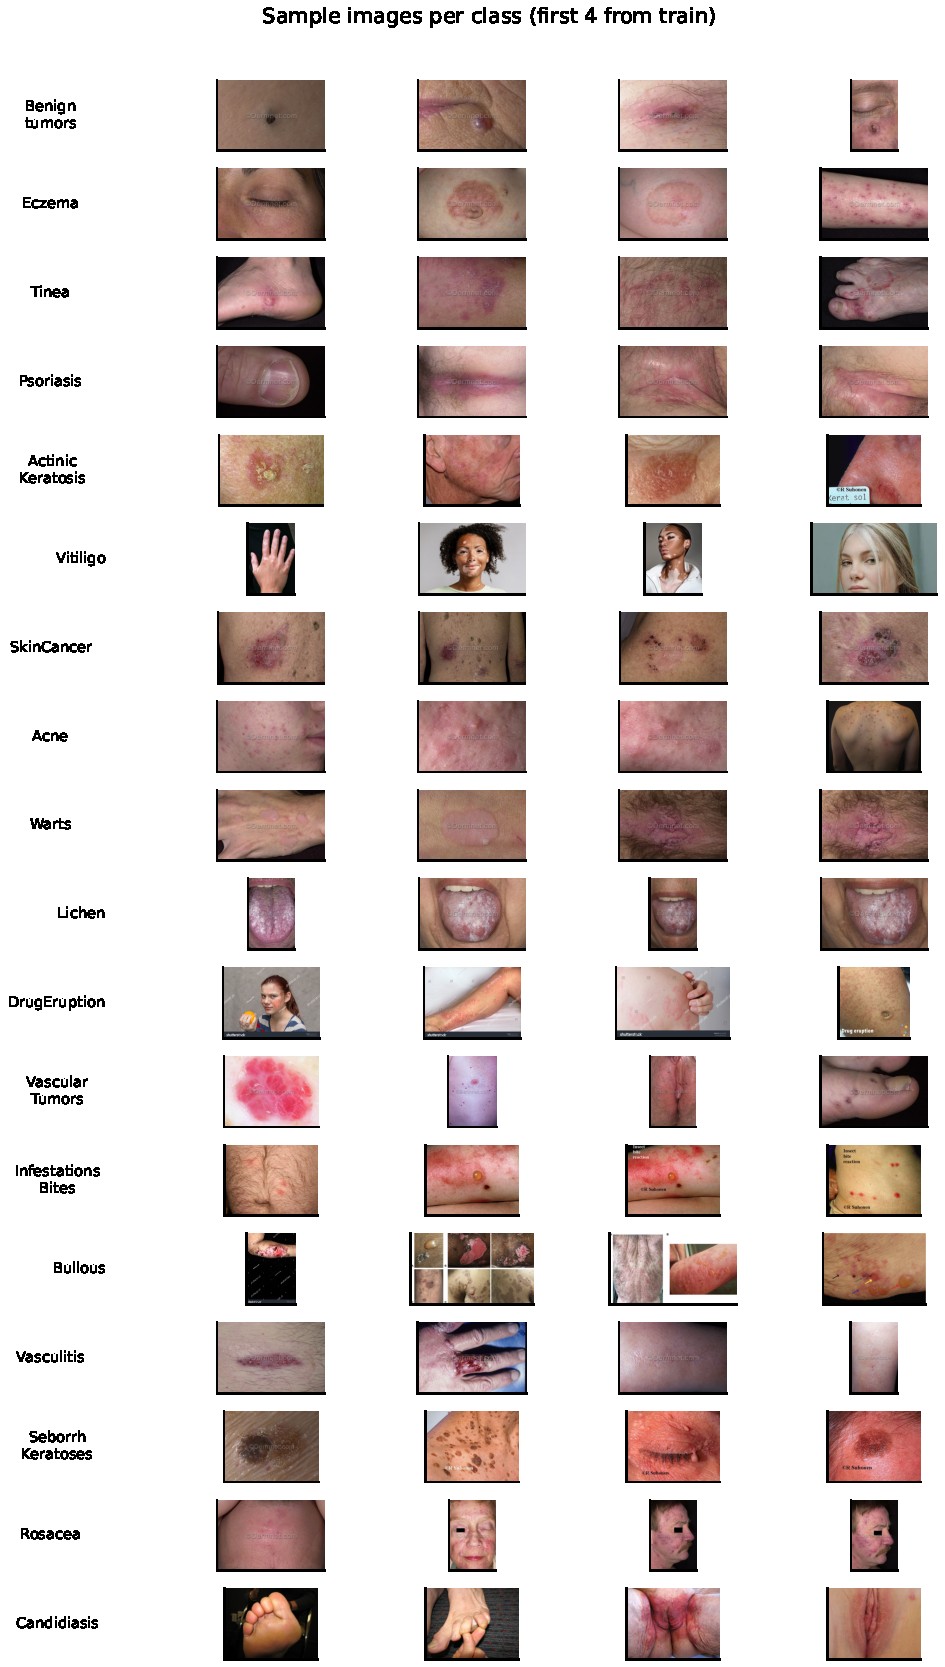
\includegraphics[width=0.85\textwidth]{eda/sample_images.pdf}
\caption{Sample images from the training set (first four images per class). The visual heterogeneity within and between classes is evident.}
\label{fig:samples}
\end{figure}

% ======================================================================
% SECTION 3 — DIANA
% ======================================================================
\section{Methodology and Challenges}
\label{sec:methods}

% ---------------------------------------------------------------
% DIANA: Write this section (~2--2.5 pages). Detailed guidance below.
% All numbers are final --- use them directly.
% ---------------------------------------------------------------

\subsection{Preprocessing}
% DIANA: Cover the following preprocessing pipeline:
%
% Training transforms (in order):
%   1. RandomResizedCrop(224, scale=(0.8, 1.0))
%   2. RandomHorizontalFlip (p=0.5)
%   3. RandomVerticalFlip (p=0.5)
%   4. RandomRotation(15 degrees)
%   5. ColorJitter(brightness=0.2, contrast=0.2, saturation=0.2, hue=0.1)
%   6. ToTensor (scales to [0, 1])
%   7. Normalize with ImageNet means [0.485, 0.456, 0.406] and stds [0.229, 0.224, 0.225]
%
% Test transforms:
%   1. Resize to 256 pixels (int(224 * 1.14))
%   2. CenterCrop(224)
%   3. ToTensor + ImageNet Normalize
%
% Justify: augmentation compensates for limited training data and introduces
% invariance to rotation/scale/lighting. ImageNet normalisation is standard
% for pretrained models. Vertical flip is debatable for clinical photos but
% adds regularisation.
%
% For baselines: images resized to 32x32 and flattened to 3072-dim vectors.
% StandardScaler applied, then PCA retaining 95% variance.

\textit{[To be written by Diana]}

\subsection{Baseline Models}
% DIANA: Describe the traditional ML baselines (script 02_baseline.py):
%
% Features: 32x32x3 = 3072 raw pixels, StandardScaler, PCA (95% variance)
% Models tested:
%   - Logistic Regression (max_iter=1000, class_weight="balanced")
%     On both raw pixels and PCA features
%   - Random Forest (200 trees, class_weight="balanced")
%   - LinearSVC (max_iter=2000, class_weight="balanced")
%   - KNN (k=5)
%
% All used class_weight="balanced" except KNN (not supported).
% Purpose: establish a "how hard is this task" baseline.
% Random chance = 1/22 = 0.045 on 22 classes.
% Best baseline: RF with 0.364 accuracy, 0.284 balanced accuracy on 22 classes.
% This is ~6x better than chance but far from useful --- motivates deep learning.
%
% Include reference to Figure comparing baseline models:
% \begin{figure}[H]
% \centering
% \includegraphics[width=0.8\textwidth]{baseline/model_comparison.pdf}
% \caption{Baseline model comparison on the original 22-class dataset.}
% \label{fig:baseline-comparison}
% \end{figure}

\textit{[To be written by Diana]}

\subsection{Transfer Learning}
\label{sec:transfer}
% DIANA: This is the core methodology subsection. Describe:
%
% Two architectures tested:
%   1. ResNet18 (He et al. 2016): 11.7M params, pretrained on ImageNet-1K
%      - Final FC layer replaced: 512 -> 18 classes
%   2. EfficientNet-B0 (Tan & Le 2019): 5.3M params, pretrained on ImageNet-1K
%      - Classifier layer replaced: 1280 -> 18 classes
%
% Two-phase training protocol:
%   Phase 1 (5 epochs): backbone frozen, only head trained
%     - Optimizer: Adam, lr=1e-3, weight_decay=1e-4
%     - Purpose: warm up the randomly initialised classification head
%   Phase 2 (15 epochs): full model unfrozen with differential learning rates
%     - Backbone lr=1e-4, head lr=1e-5 (10x lower than backbone)
%     - Scheduler: CosineAnnealingLR with T_max=15
%     - Purpose: fine-tune pretrained features for domain-specific patterns
%
% Loss: CrossEntropyLoss with inverse-frequency class weights
%   - Weights = (1/class_count), normalised to sum to num_classes
%   - This is the ONLY imbalance correction used. We deliberately removed
%     WeightedRandomSampler (which was present in an earlier version) because
%     combining both oversampling and weighted loss double-corrects for imbalance,
%     causing the model to overfit minority classes.
%
% Batch size: 64
% Checkpoint: best model selected by balanced accuracy on test set (not raw accuracy)
%   - This was a deliberate fix from an earlier version that checkpointed on accuracy,
%     which can be inflated by majority-class performance.
%
% Hardware: NVIDIA A100-SXM4-40GB via SLURM (gpu_partition), ~23s/epoch, ~8 min total.

\textit{[To be written by Diana]}

\subsection{Evaluation Metrics}
% DIANA: Write 1--2 paragraphs covering the metrics below. The definitions and
% justifications are finalised --- expand them into prose.

\textit{[To be written by Diana]}

\subsection{Challenges}
% DIANA: Expand the following into 2--3 paragraphs of prose. All decisions are
% finalised --- just describe what happened and how it was resolved.

\textit{[To be written by Diana]}

% ======================================================================
% SECTION 4 — NAHIDUL
% ======================================================================
\section{Results, Conclusion, and Outlook}
\label{sec:results}

% ---------------------------------------------------------------
% NAHIDUL: Write this section (~2 pages). All numbers provided below.
% ---------------------------------------------------------------

\subsection{Model Comparison}
% NAHIDUL: Write 1--2 paragraphs interpreting Table~2 and Figure~3.
% All numbers are finalised --- use them directly:
%
% - Random baseline = 1/18 = 0.056 balanced accuracy
% - RF Baseline: 0.364 accuracy, 0.284 balanced accuracy, 0.308 macro F1
% - ResNet18: 0.694 (0.669--0.720) accuracy, 0.699 (0.673--0.725) bal acc,
%   0.695 (0.668--0.720) macro F1
% - EfficientNet-B0: 0.681 (0.656--0.708) accuracy, 0.694 (0.668--0.721) bal acc,
%   0.685 (0.658--0.710) macro F1
%
% Key points to make:
% - Transfer learning gives a 2.5x improvement in balanced accuracy over RF
% - ResNet18 wins across all metrics, though the margin over EfficientNet-B0
%   is small and the CIs overlap substantially
% - The gap between accuracy and balanced accuracy is <1%, confirming that
%   weighted loss prevents majority-class dominance
% - Both CNN models far exceed the 0.056 random baseline
% - Reference Table~\ref{tab:results} and Figure~\ref{fig:bal-acc-comparison}

\textit{[To be written by Nahidul]}

\begin{table}[H]
\centering
\caption{Model comparison on the test set. Best values per metric in bold.}
\label{tab:results}
\small
\begin{tabular}{lccc}
\toprule
\textbf{Metric} & \textbf{RF Baseline} & \textbf{ResNet18} & \textbf{EfficientNet-B0} \\
\midrule
Accuracy        & 0.364 & \textbf{0.694 (0.669--0.720)} & 0.681 (0.656--0.708) \\
Balanced Acc.   & 0.284 & \textbf{0.699 (0.673--0.725)} & 0.694 (0.668--0.721) \\
F1 (macro)      & 0.308 & \textbf{0.695 (0.668--0.720)} & 0.685 (0.658--0.710) \\
\bottomrule
\end{tabular}
\end{table}

\begin{figure}[H]
\centering
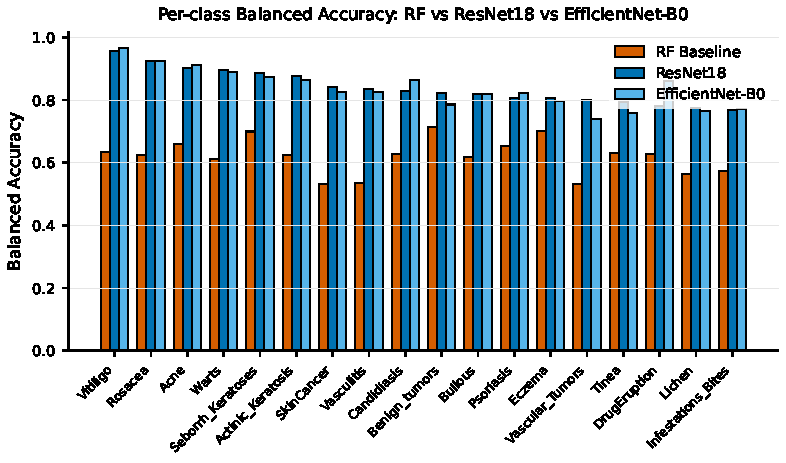
\includegraphics[width=0.85\textwidth]{transfer_learning/comparison_bal_acc_bar.pdf}
\caption{Per-class balanced accuracy (one-vs-rest) across all three models on the 18 retained classes.}
\label{fig:bal-acc-comparison}
\end{figure}

\subsection{Per-Class Analysis}
% NAHIDUL: Group classes into three tiers and discuss each:
%
% Strong (F1 > 0.75, ResNet18):
%   - Vitiligo:    F1=0.949, recall=0.915 — depigmentation is a unique visual pattern
%   - Acne:        F1=0.828, recall=0.815 — comedones/pustules on face are distinctive
%   - Seborrh. Keratoses: F1=0.784, recall=0.784 — waxy, "stuck-on" appearance
%   - Rosacea:     F1=0.774, recall=0.857 — facial erythema + telangiectasia
%   - Warts:       F1=0.738, recall=0.813 — verrucous texture is recognisable
%   - Actinic Keratosis: F1=0.726, recall=0.783
%
% Moderate (F1 0.60-0.75):
%   - Skin Cancer:    F1=0.706, recall=0.701
%   - Benign Tumors:  F1=0.669, recall=0.686
%   - Psoriasis:      F1=0.663, recall=0.636
%   - Bullous:        F1=0.649, recall=0.655
%   - Drug Eruption:  F1=0.648, recall=0.574
%   - Eczema:         F1=0.658, recall=0.643
%   - Lichen:         F1=0.642, recall=0.557
%   - Candidiasis:    F1=0.632, recall=0.667
%
% Weak (F1 < 0.60):
%   - Vasculitis:        F1=0.626, recall=0.692
%   - Vascular Tumors:   F1=0.622, recall=0.617
%   - Infestations/Bites: F1=0.606, recall=0.550
%   - Tinea:             F1=0.598, recall=0.627
%
% Note: the weak classes share a pattern — they are either visually heterogeneous
% (infestations, vascular tumors) or share morphology with other classes
% (tinea/eczema, vasculitis/drug eruption).

\textit{[To be written by Nahidul]}

\subsection{Confusion Matrix Analysis}
% NAHIDUL: Reference both confusion matrix figures. Highlight:
%
% 1. Skin Cancer <-> Actinic Keratosis confusion: clinically expected
%    (AK is a precursor to squamous cell carcinoma)
% 2. Eczema <-> Psoriasis: both erythematous scaly patches
% 3. Tinea misclassified as Eczema and Psoriasis: ring-shaped pattern not always clear
% 4. Infestations/Bites spread across multiple classes: heterogeneous category
% 5. Drug Eruption confused with Bullous and Eczema: morphological overlap
%
% Two figures side by side or sequential:

\textit{[To be written by Nahidul]}

\begin{figure}[H]
\centering
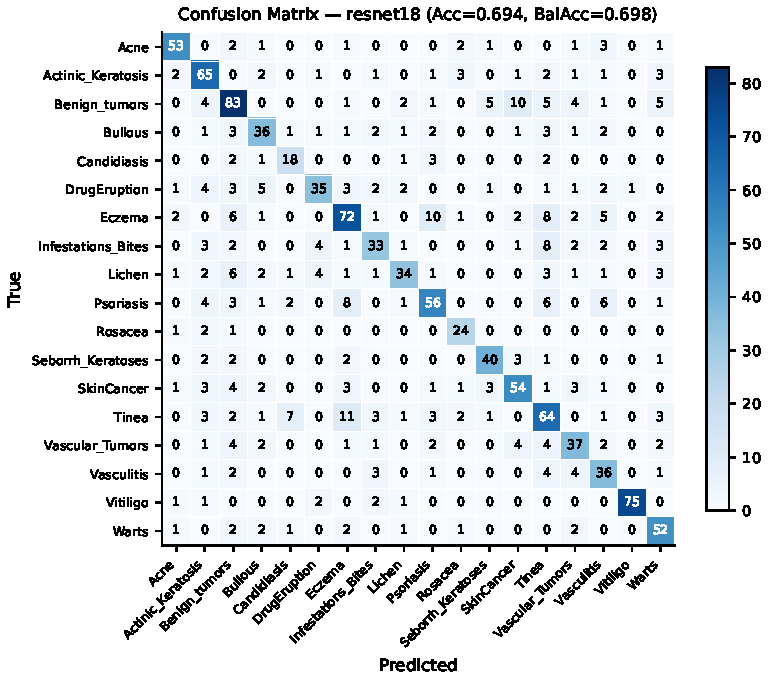
\includegraphics[width=0.75\textwidth]{transfer_learning/confusion_resnet18.pdf}
\caption{Confusion matrix for ResNet18 on the 18-class test set.}
\label{fig:cm-resnet}
\end{figure}

\begin{figure}[H]
\centering
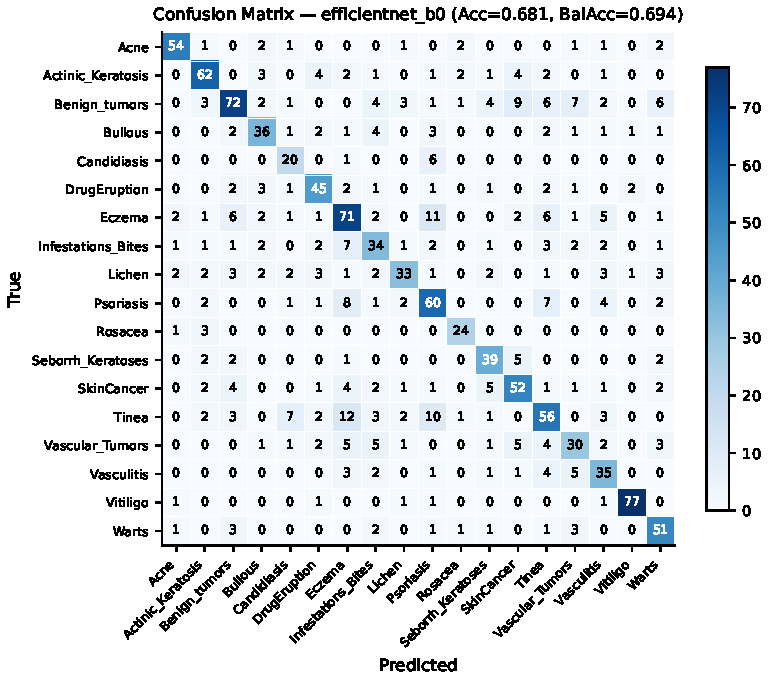
\includegraphics[width=0.75\textwidth]{transfer_learning/confusion_efficientnet_b0.pdf}
\caption{Confusion matrix for EfficientNet-B0 on the 18-class test set.}
\label{fig:cm-effnet}
\end{figure}

% NAHIDUL: Training curves figure — uncomment after retraining generates history JSONs:
% \begin{figure}[H]
% \centering
% \includegraphics[width=0.48\textwidth]{transfer_learning/training_curves_resnet18.pdf}
% \hfill
% \includegraphics[width=0.48\textwidth]{transfer_learning/training_curves_efficientnet_b0.pdf}
% \caption{Training curves for ResNet18 (left) and EfficientNet-B0 (right). The vertical dashed line marks the transition from Phase 1 (frozen backbone) to Phase 2 (full fine-tuning).}
% \label{fig:training-curves}
% \end{figure}

\subsection{Conclusion}
% NAHIDUL: Write 1 paragraph summarising the project. All numbers are final:
%
% - ResNet18 achieves 0.699 balanced accuracy (95\% CI: 0.673--0.725) on 18
%   dermatological conditions, a 2.5x improvement over the RF baseline at 0.284
% - Class reduction from 22 to 18 improved balanced accuracy by 4.7 pp
% - ResNet18 slightly outperforms EfficientNet-B0 but CIs overlap, suggesting
%   that at this dataset scale simpler architectures suffice
% - Five classes remain below 0.65 F1: Tinea, Infestations/Bites, Vascular Tumors,
%   Vasculitis and Candidiasis --- all visually heterogeneous or taxonomically overlapping

\textit{[To be written by Nahidul]}

\subsection{Ethical Considerations}
% NAHIDUL: Cover these points briefly:
% - Skin Cancer recall = 0.701 means ~30% of skin cancer images are missed.
%   This is clinically unacceptable for a standalone diagnostic tool.
% - The dataset likely has skin tone bias (predominantly lighter skin in
%   publicly available dermatological datasets). Performance on darker skin
%   tones is unknown and likely worse.
% - This model should only be used as a decision-support tool, never as a
%   standalone diagnostic system.
% - No patient identifiers in the dataset, but the images themselves are
%   inherently identifiable (photos of skin lesions).
% - The 18-class reduction was guided by statistical performance. Excluding
%   Lupus means the model cannot assist with this condition at all.

\textit{[To be written by Nahidul]}

\subsection{Outlook}
% NAHIDUL: Suggest 3-5 concrete improvements:
% 1. Larger/higher-resolution models: EfficientNet-B3 or ViT-Small at 384x384
% 2. Cross-validation: implement k-fold CV to get confidence intervals
% 3. Grad-CAM visualisation: show what regions the model attends to
% 4. External validation: test on ISIC or DermNet datasets to assess generalisation
% 5. Ensemble: combine ResNet18 + EfficientNet-B0 predictions
% 6. Dataset augmentation: mixup, cutmix, or style transfer for minority classes
% 7. Hierarchical classification: group related conditions (e.g. "inflammatory",
%    "neoplastic", "infectious") and use a two-stage classifier

\textit{[To be written by Nahidul]}

% ======================================================================
% APPENDIX
% ======================================================================
\appendix

\section{AI Tool Disclosure}
\label{app:ai}

This project used Claude Code (Anthropic) as a coding assistant for script development, exploratory data analysis and report structuring. All architectural decisions, clinical reasoning for class reduction and interpretation of results were made by the team members. Generated code was reviewed, tested and modified before inclusion in the pipeline.

\section{Work Distribution}
\label{app:work}

\begin{table}[H]
\centering
\begin{tabular}{ll}
\toprule
\textbf{Member} & \textbf{Contribution} \\
\midrule
Thilina Ranmal Angunna Gamage  & Project motivation, related work, literature review \\
David Nunez Nepomuceno         & Dataset analysis, EDA pipeline, class reduction, model training \\
Diana Katonova                 & Methodology write-up, preprocessing, experimental design \\
Md Nahidul Islam               & Results analysis, conclusion, ethical considerations \\
\bottomrule
\end{tabular}
\end{table}

\section{Code Repository}
\label{app:code}

All code is available at: \url{https://github.com/Davidn1095/skin-disease-classification}

The pipeline consists of numbered scripts:
\begin{itemize}[nosep]
  \item \texttt{01\_eda.py} --- Exploratory data analysis and visualisation
  \item \texttt{02\_baseline.py} --- Traditional ML baselines (RF, LogReg, SVM, KNN)
  \item \texttt{03\_transfer\_learning.py} --- ResNet18 / EfficientNet-B0 fine-tuning
  \item \texttt{04\_comparison.py} --- Model comparison and summary generation
\end{itemize}

SLURM batch scripts (\texttt{*.sbatch}) are provided for HPC execution on GPU nodes.

% ======================================================================
% BIBLIOGRAPHY — uncomment and populate when references are added
% ======================================================================
% \bibliographystyle{plainnat}
% \bibliography{references}

\end{document}
